\documentclass[12pt]{hdxthesis}  % default square logo 

%load any additional packages
\usepackage{amssymb}
\usepackage{xspace}
\usepackage{url}
\usepackage{caption}
\usepackage{listings}
\lstset{
basicstyle=\small\ttfamily,
columns=flexible,
breaklines=true
}

\newcommand{\etal}{\emph{et al.}\xspace}
\newcommand{\argmax}{\mathop{\mathrm{argmax}}\nolimits}
%input macros (i.e. write your own macros file called mymacros.tex 
%and uncomment the next line)
%\include{mymacros}

\title{\LARGE Kinyarwanda | English Translator\\[1ex]     %your thesis title,
       \Large A Statistical Machine Learning Approach}  %note \\[1ex] is a line break in the title

\author{Patrick Niyongabo}             %your name
\college{Hendrix College}  %your college

%\renewcommand{\submittedtext}{change the default text here if needed}
\degree{Bachelor of Arts in Computer Science}     %the degree
\degreedate{May 2017}         %the degree date

%end the preamble and start the document
\begin{document}

%this baselineskip gives sufficient line spacing for an examiner to easily
%markup the thesis with comments
\baselineskip=18pt plus1pt

%set the number of sectioning levels that get number and appear in the contents
\setcounter{secnumdepth}{3}
\setcounter{tocdepth}{3}

% added from http://tex.stackexchange.com/questions/5223/command-for-argmin-or-argmax/284054#284054
%\DeclareMathOperator*{\argminA}{arg\,min} % Jan Hlavacek % thin space, limits underneath in displays

\maketitle                  % create a title page from the preamble info
\begin{dedication}

I dedicate this thesis to my four young sisters: \newline Janvi$\grave{e}$re, Joseline, Josiane, and Fortune. I miss y'all!
%I dedicate this to you.

%I dedicate this thesis to everyone in my life.


%I dedicate this thesis to everyone who has made an influence on my LIFE. 

%To my four young sisters: Janvi$\grave{e}$re, Joseline, Josiane, and Fortune, I miss you. 

%To my father and mother, I can't thank you for everything yo have done for me. Hope to see you soon.

%To everyone in my life, I dedicate this one to you.


%https://github.com/moses-smt/mosesdecoder/tree/master/scripts/share/nonbreaking_prefixes


%http://stackoverflow.com/questions/27669446/statistical-machine-translation-from-hindi-to-english-using-moses

%http://tex.stackexchange.com/questions/3587/how-can-i-use-bibtex-to-cite-a-web-page


\end{dedication}        % include a dedication.tex file
\begin{acknowledgements}
My deep gratitude goes to my thesis advisor, Dr. Gabriel Ferrer for his patience and guidance. I would also like to take this moment to thank every faculty member of the Hendrix College Math and Computer Science department for their relentless support. To all students and other friends who helped me or encouraged me in any way when I was working on this project, I can only say thank you!    
\end{acknowledgements}   % include an acknowledgements.tex file
\begin{abstract}
Statistical  Machine  Translation  (SMT)  is  a  statistical machine  learning (SML) technique that uses statistical models to generate translations from one language to another. In this paper, I describe the statistical machine translation (SMT) approach that I am using to make an English to Kinyarwanda translator, and explain the phrase-based model used in some of the most prominent SMT systems such as Cdec, Joshua, and Moses. The latter SMT system being the one I am using to develop my English to Kinyarwanda translation model.
\end{abstract}          % include the abstract

\begin{romanpages}          % start roman page numbering
\tableofcontents            % generate and include a table of contents
\listoffigures              % generate and include a list of figures
\end{romanpages}            % end roman page numbering

%now include the files of latex for each of the chapters etc
\chapter{Introduction}

In recent years, due to an increase in the use of mobile phones and Internet around the World\cite[p. 131-133]{quinn1987impacts}, some developing nations are turning to a technology-based services industry with the hope that technology, and the Internet in particular, will serve as tools to speed up their economic growths towards sustainable development\cite{lall1998market}. However this has proven to be a difficult challenge for countries whose popular, and in most cases, official languages are not widely used elsewhere around the World. 

The reason why this is a big issue is because even though there is a lot of free and easily-accessible information on the Internet, around $77.9\%$ of the content on the web is in the top ten most popular languages (English, Chinese, Spanish, Arabic, Portuguese, Japanese, Malay, Russian, French, and German)\cite{internetworldstats}. Therefore without the use of a translator, the information on the Internet is inaccessible, and somewhat useless, to people who can't read or understand at least one of these popular languages. 

As an example, the Rwandan government, as part if its Vision 2020 plan, wanted to implement educational initiatives that would take advantage of free resources available on the Internet but most of these initiatives have been hindered by the fact that almost $90\%$ of Rwandans are only proficient in Kinyarwanda\cite{Samuelson2010} and there doesn't exist a competent translation service that can be used to translate to (or from) Kinyarwanda.  As a Rwandan, after realizing this, I felt inclined to do something, I decided to explore possible technical solutions that could be used as a starting point in order to deal with this particular problem of information scarcity caused by linguistic barriers.

My first step when embarking on this project was to search around and see if there is any other work that has been done in this domain and to find out if there are any already-developed tools that I could use to translate any of the popular language to Kinyarwanda or vice-versa. After failing to find any competent service that supported Kinyarwanda translation\footnote{Kinyarwanda is one the langauges currently in development at Google Translate, but it is not clear whether it will be one of the supported languages anytime soon\cite{googletranslatecommunity}.}, I started looking for research being done in the domain of natural language translation, and that is how I found out about Statistical Machine Translation (SMT) systems. 

Before diving into the actual process of making a Kinyarwanda | English translator, I researched and tried out some of the freely-available SMT systems such as Moses (a complete SMT system), Cdec (a Python-based SMT decoder and aligner), and Joshua (a java-based SMT decoder). 

For building my model, I ended up using Moses for reasons discussed in my concluding remarks. In the process, I also learnt about the phrase-based model that is used heavily in the field of statistical machine translation\cite{koehn2003statistical}. In this paper, I will explain how that model works and how it is implemented and how it is used in the above-mentioned SMT systems, while focusing on Moses and its role in my project. % introduction
\chapter{Statistical Machine Translation}
Even though there are many ways that translation from one language to another can be done\cite[p. 5-6]{trujillo2012translation}, many machine translation (MT) scholars now consider statistical machine translation (SMT) as the most effective way for developing efficient large-scale translation systems\cite[p. xi]{koehn2009statistical}. The main idea behind SMT is to use large text translations from one language to another (parallel corpora) to generate translation tables, and then use good-quality content (monolingual corpus) of the target language to train its model, that is teaching the system about the general structure of that particular language so that is the system is able to evaluate generated translations and pick the most likely among them by using set statistical parameters.

To produce a good translation model, you need to have a large dataset of parallel corpora of high quality to use when developing translation rules for your model. According to Franz Josef Och, an SMT pioneer who created started the Google Translate project, you need at least a parallel corpora of 50-200 million words\cite{och2005statistical}.  You also need to have a very large monolingual corpus, more than a billion words according to Och, to use when training the target language model\cite{och2005statistical}. In addition to this you have to \textit{tune} the translation model. \textit{Tuning} is the process in which the translation performance of the model is optimized by using a different parallel corpus that is of greater or equal quality than the one that that was used in the training stage. Given these two, and other, steps involved in developing an SMT system heavily employ statistical machine learning techniques, it is only reasonable that I discuss the basics of statistical machine learning before diving into the specifics of SMT systems. 

\section{Statistical Machine Learning}

After the development of digital computers during the last half of the $20^{th}$ century, there have been multiple attempts of using machines to perform several tasks such as speech recognition, text translation, and data analysis. The process of teaching a machine the basics how to perform a certain task, and then letting the machine learn the rest on its own, is called ``machine learning''\cite{princetonml}.

Statistical machine learning is a branch of machine learning that uses data to generate statistical models that can then be used as functions when modeling new data inputs. To develop an SMT system, one uses large amounts of corresponding texts from both the source language and the target language as inputs of a learning algorithm that then generates statistics of equivalence between the two bodies of texts in form of probabilities. These probabilities are then used as inputs of another program that does the actual translation. 

The resulting translating system can take a string of text in the source language and uses the rules, in this case statistical probabilities generated by the first algorithm, to output the best possible translation according to its rules. This is a very simplified example as it doesn't include all the steps involved in training an SMT model using prominent SMT systems such as Moses\cite{koehn2007moses}, but it provides enough details to showcase how basic concepts from machine learning are applied and used by SMT systems and SMT-based translation models. 
\section{The Mathematics of Machine Translation}
%%%%%%%%%%%%%%%%%%%%%%%%%%%%%%%%%%%%%%%%%%%%%%%%%%%%%%%%%%
In this section, I explore the Mathematics behind some of the main SMT concepts as discussed in an article by Brown \etal entitled \textit{``The Mathematics of Statistical Machine Translation: Parameter Estimation''}\cite{brown1993mathematics}.
\subsection{Probabilities in Translation}
Suppose we are given an English sentence $e$, and we are trying to translate it to its corresponding Kinyarwanda sentence $k$, $P(k|e)$ is the probability that we will get the Kinyarwanda translation $k$ when starting with the English sentence $e$. $P(k)$ is the prior probability that $k$ happens based on our system's Kinyarwanda language model. $p(e,k)$ is the joint probability that both $e$ and $k$ happen. If a Kinyarwanda sentence $k$ is the output of our English to Kinyarwanda translator when English sentence $e$ is the input, it is clear that $e$ and $k$ are related (not independent), therefore their chances of happening depend on each other. Thus,
\begin{equation}\label{zero1}
P(e,k) = P(e) * P(k|e)
\end{equation}
In the same fashion,
\begin{equation}\label{zero2}
P(e,k) = P(k) * P(e|k)
\end{equation}
The  above two equations can be combined to get the Bayes' Theorem equation:
\begin{equation}\label{one}
P(k|e) = \frac{P(k)P(e|k)}{P(e)}
\end{equation}
The goal of the English to Kinyarwanda translation system is to return the best translation, that is finding the translation $k_{best}$ that maximizes the probability $P(k|e)$ for any given input English sentence $e$ as shown in the equation below:
\begin{equation}
\argmax_e(P(k|e)) = \argmax_e(P(k)P(e|k))\\
\end{equation}
Notice that $P(e)$ is eliminated in equation $2.4$ as it is a constant. The probability that sentence $e$ is in English doesn't change as we go through the translation process because $e$ it is the sentence we are trying to translate. Now that we have equation $2.4$ that maximizes $P(k|e)$, we can use it to learn more about how our English to Kinyarwanda translation model works. As an example, let's say we want to use our English to Kinyarwanda SMT-based model to translate the English sentence: ``\textit{cats and dogs are both mammals}''. To translate this sentence, our translation model would have to go through these important three steps:

\begin{enumerate}
    \item Use a trained translation system to generate all possible Kinyarwanda translations.\footnote{This can be done using an SMT system such as Moses. The process of training and using a bilingual translation system using Moses is explained in Chapter 3.}
    \item For each Kinyarwanda translation, k, calculate:
    \begin{itemize}
        \item $P(k)$, the prior probability that k is indeed a Kinyarawnda sentence.
        \item $P(e|k)$, the reverse probability that if we started with the Kinyarwanda sentence $k$, we would get $e$, the English sentence that we are trying to translate.
        \item Calculate the product of $P(k)$ and $P(e|k)$.
    \end{itemize}
    \item Output $k_{best}$, that is the sentence $k$ that has the biggest $p(k|e)$. Remember that from equation $2.4$, when maximized, $p(k|e)$ is equivalent to the maximized product of $p(k)$ and $p(e|k)$ as $p(k)$ doesn't change during the translation process.
\end{enumerate}
\begin{figure}[h]
\begin{center}
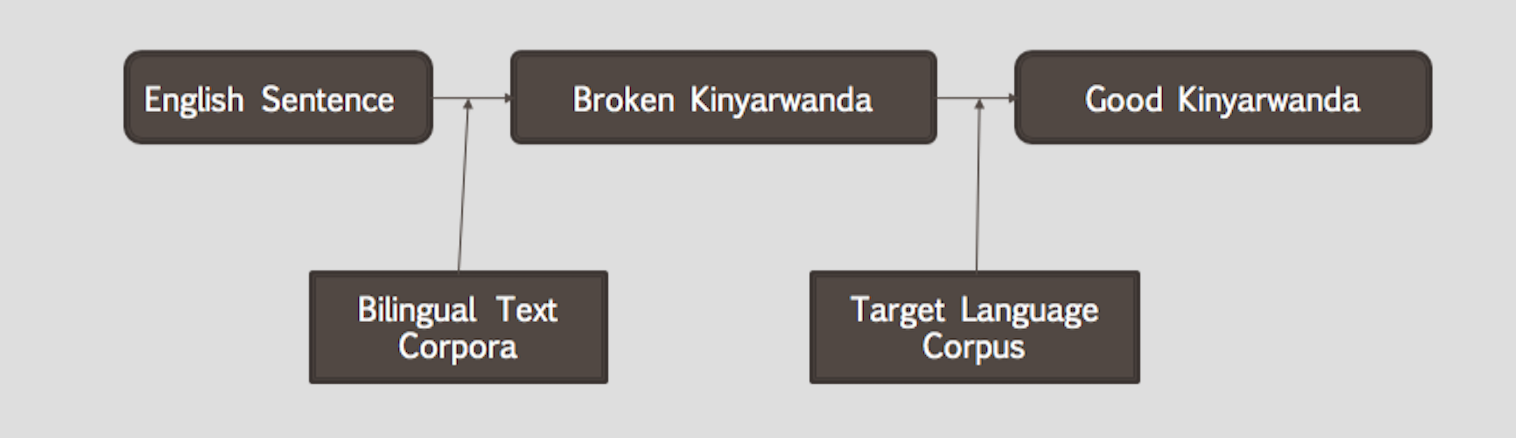
\includegraphics[width=4in]{figures/smt_works.png}
\caption{An illustration of how SMT works. A graphical representation of equation $2.4$.}
\end{center}
\end{figure}

As it can be seen from the above example, Equation $2.4$ is very important. In their article, Brown \textit{et al.} described it as the ``Fundamental Equation of Machine Translation''\cite[p. 265]{brown1993mathematics} as it is capable of summarizing all the three steps involved in translating any given sentence from one language to another by using an SMT-based translation model.

At this point I will focus on the second step of the above-described process as the first and third steps can be easily implemented by a computer program that has access to the date of both the translation model and the target language model, and these two models can be generated by using an SMT system such as Moses in a process that I describe in chapter 3. However before addressing step $2$, let's go back and ask one important question. \textbf{Why is it even necessary to to care about $P(k)*P(e|k)$? Can't we just directly calculate $P(k|e)$ if all we are trying to find is the Kinyarwanda sentence $k_{best}$ that maximize the value of $P(k|e)$?}

Well the answer to that question is rather a devious one. To understand it, we have to look at this question as if we were computer programs. A computer program whose goal is to output the best possible translation $k$ when given an English input sentence $e$ will only care about two things: 
\begin{enumerate}
\item The quality of the output sentence $k$ in the target language (Kinyarwanda in this example).
\item The connection of that output sentence $k$ to the input sentence $e$ that it started with, that is how related are $e$ and $e$ compared to other sentence pairs seen by the translation model in the training and tuning stages.
\end{enumerate}

However, unlike humans, a computer program can't just look at a sentence and decides if it is of good Kinyarwanda quality. It can't also deduce, by just looking at two or more Kinyarwanda sentences, which one is the better translation for a given English sentence. Thus, when in a situation like this, a computer program must reason backwards. At least this is how SMT-based systems are programmed to handle tasks like this one. As long the translation system has access to the translation tables from which it can generate several translations, and assigns to each one of them an exact conditional probability that if we started with that translation, and used the same translation system only going backwards, that is from the target language to the source language, we would get the original English sentence $e$ that we are trying to translate to Kinyarwanda. That conditional probability, combined with the prior probability $p(k)$, enables the translation system to maximize the chance of getting the best possible translation $k$.


For example, the correct Kinyarwanda translation of the English sentence $(e)$: ``\textit{cats and dogs are both mammals}'', is $(k)$: ``\textit{injangwe n' imbwa ni inyamabere zombi}'', with cats = injangwe, and = n', dogs = imbwa, are = ni, both = zombi, mammals = inyamabere. However, we can imagine that our translator, being very smart as it is, may generate the following translation: ``\textit{injangwe n' imbwa ni 
\underline{inyamaswa} zombi}'' $(k')$, which is the translation to ``\textit{cats and dogs are both \underline{animals}}''$(e')$. So even though translation $(k')$ is a good-structured and grammatically-correct Kinyarwanda sentence and would have a high $P(k')$, it is not the correct translation of $(e)$, so its conditional probability, $P(e|k')$, would be low, thus lowering the overall chance that sentence $(k')$ is going to picked as the output by the translator. 

\begin{figure}[h]
\begin{center}
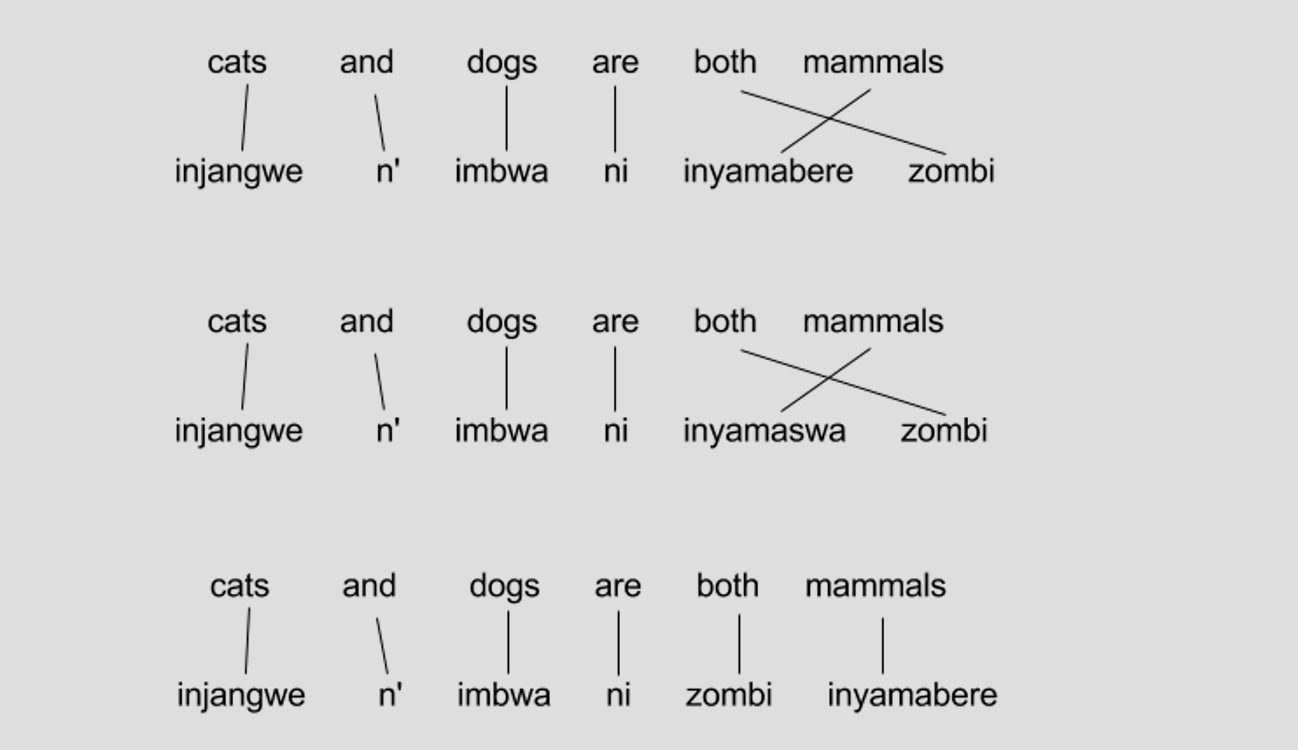
\includegraphics[width=4in]{figures/cats.png}
\caption{Comparison of several possible Kinyarwanda translations of the same English sentence: ``\textit{cats and dogs are both mammals}''.}
\end{center}
\end{figure}
On the other hand, we can imagine a misaligned version of sentence $k$. An example of this case is a sentence like ``\textit{injangwe n'imbwa ni zombi inyamabere}''$(k'')$ which is a one-to-one translation of sentence $(e)$ with each word with the words being in the same posistion as they were previously in $e$. Sentence $k''$ would likely be judged by the translation model as a very good translation. However, if our translation system's Kinyarwanda model was good enough, it would detect the inconsistency in the order of words in $(k'')$ compared to other Kinyarwnda sentences, and $P(k'')$ would be low compared to $P(k)$; however training SMT language models to be very good at detecting minor inconsistencies like this one requires large (more than a billion words) monolingual corpora\cite{och2005statistical}. %An alternative way of addressing this particular common issue of incorrect reordering of words is having a distinct alignments model that is later added to the language model to make sure that cases like the one in the above-mentioned example is correctly dealt with by the translation system. 

Back to our English to Kinyarwanda translation model, we can see that even though the combination of $P(k)$ and $P(e|k)$ is used to make sure that the results of our translation system is as correct as it can get, we can imagine some instances in which the two probabilities may contradict each other, that is when a bigger $P(k)$ means getting a lower $P(e|k)$ or vice versa. In these cases, it is recommended to add weight coefficients to equation $2.3$. Added coefficients depend on the data used in the training and tuning stages, and on the structure of the languages being dealt with.
%%%%%%%%%%%%%%%%%%%%%%%%%%%%%%%%%%%%%%%%%%%%%%%%%%%%%%%%%%%%%%%%%%%%%%%%%%%%%%%%%%%%%%%%%%%%%%%%%%%%%%%%%%%%%%%%%%%%%%%%%%%%%%%%%%%%%%%%%%%%%%%%%%%%%%%%%%%%%%%%%%%%%
\subsection{Alignments}
%%%%%%%%%%%%%%%%%%%%%%%%%%%%%%%%%%%%%%%%%%%%%%%%%%%%%%%%%%%%%%%%%%%%%%%%%%%%%%%%%%%%%%%%%%%%%%%%%%%%%%%%%%%%%%%%%%%%%%%%%%%%%%%%%%%%%%%%%%%%%%%%%%%%%%%%%%%%%%%%%%%%%

As different languages have different structures, and one word from the source language can be translated using zero, one, or multiple words in the target language, it is important that we account for all these possibilities caused by changes in both the structure, and the \textit{fertility} of words in, the language pairs we are working with. The \textit{fertility} of a word is defined as the number of words that are generated by that particular word  when translated from one language to another. To better understand this let's use the following example of a Kinyarwanda - English sentence pair. 
\begin{center}
\begin{tabular}{c}
\begin{lstlisting}
Kinyarwanda: ``Imana yirirwa ahandi igataha i Rwanda.''
English: ``God spends the day elsewhere but spends the night in Rwanda.''
\end{lstlisting}
\end{tabular}
\end{center}

From the above translation, one can immediately deduce that the Kinyarwanda words in the above sentence have higher fertility rates when being translated to English;  however, using this example and doing the translation from English to Kinyarwanda, the English words would have lower fertility rates. 

In the above example, as it can be seen in figure $2.3$, the word ``Imana'' has a fertility of $1$ as it generates one English word, ``God''. On another hand, the word ``yirirwa'' has a fertility of $3$, as it generates a total of three English words (``spends'', ``the'', ``day''). The relationship between Kinyarwanda words and English words illustrated in Figure $2.3$ can also be represented using the Brown \textit{et al.} notation\cite[p. 266]{brown1993mathematics} as following: \textit{(God spends the day elsewhere but spends the night in Rwanda $|$ Imana(1) yirirwa(2, 3, 4) ahandi(5) igataha(7, 8, 9) i(10) Rwanda(11))}. 
In this notation, the numbers in parentheses represent the indexes that the Kinyarwanda words are equivalent to. As you may have noticed, index $6$ is skipped because the English word ``but'' is not connected to any particular word in the Kinyarwanda sentence even.  It is implicitly implied with the structure of the sentence. Such words that are generated somewhat out of nowhere are called ``\textit{spurious}'' words\cite[p. 2]{Germann:2003:GDS:1073445.1073455}.  

However the opposite can also happen. We can imagine translating a Kinyarwanda sentence to English, and losing one of its words through the translation process. In that scenario, that ``\textit{lost}'' word may have been combined with another word and then translated together, or it may have been lost and just been translated through the context of the produced sentence. The ``lost'' word scenario is featured in fig $2.4$.

\begin{figure}[h]
\begin{center}
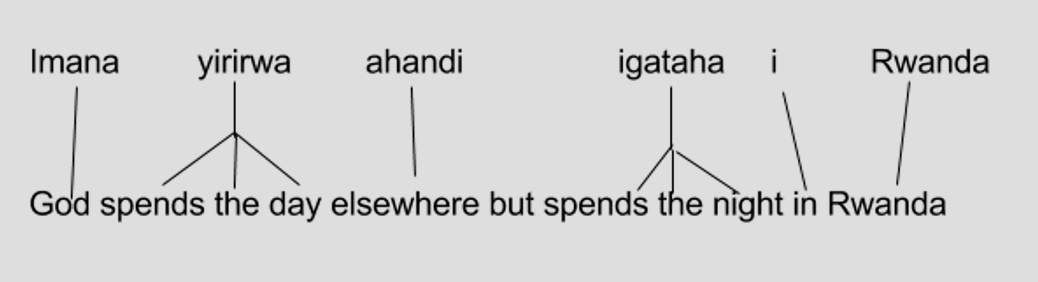
\includegraphics[width=4in]{figures/fig-one.png}
\caption{An example of sentence alignment with a ``spurious'' word: ``\textit{but}''.}
\end{center}
\end{figure}
\begin{figure}[h]
\begin{center}
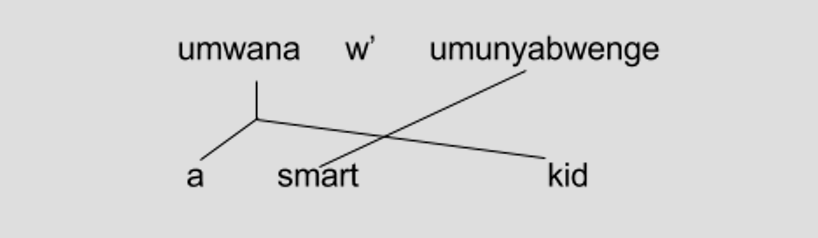
\includegraphics[width=4in]{figures/fig-two.png}
\caption{Example of a sentence alignment with a ``lost'' word: ``\textit{w'}''.}
\end{center}
\end{figure}
\begin{figure}[h]
\begin{center}
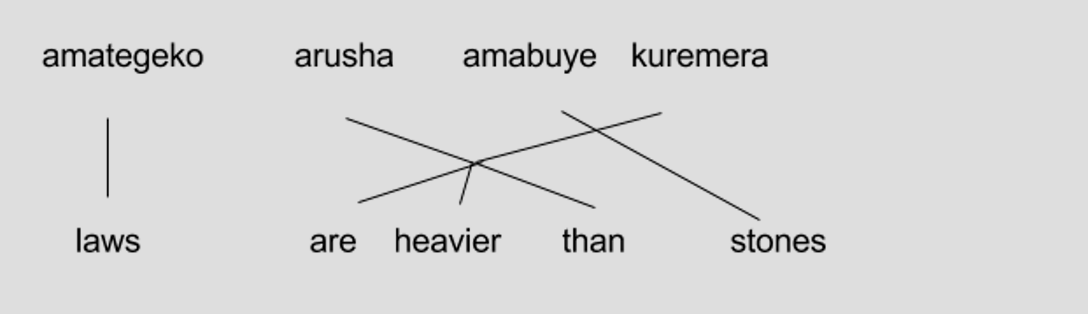
\includegraphics[width=4in]{figures/fig-three.png}
\caption{A sentence pair alignment containing both ``lost'' and ``spurious'' words.}
\end{center}
\end{figure}

However most sentence pairs that are dealt with during the training stage or the translation process do not just contain spurious words or lost words but a mixture of both (e.g.: Figure $2.5$); and that is why alignment probabilities should be assigned to these two possibilities when developing a translation model.  Depending on which language pair you are dealing with, ``lost'' and ``spurious'' words can have a very significant impact on the quality of the translation results. They ought to be taken seriously. 

According to Brown \etal\cite[p. 268]{brown1993mathematics}, the way that SMT decoders use to handle these irregular cases of alignments is by adding one empty \textit{cept}\footnote{In this case, \textit{cept} is defined as a word or a group of words whose context is translated together.} to the sentence about to be translated, and using it as an alignment partner for any ``spurious'' word found in the final translation. As for ``lost'' words, Brown \textit{at al.}\cite[p. 268]{brown1993mathematics} suggest using their implied meaning or context to align them with their closest or related counterparts in the target language sentence.


By applying these suggestions to the example illustrated in Figure $2.4$, we would get the following alternative alignment: \textit{(a smart kid $|$ $k_0$(1)  umwana(1) w'(2) umunyabwenge(2))}, where $k_0$, stand for the null cept that we placed at the beginning of the Kinyarwanda string before translating it to English. Also notice how instead of skipping the string \textit{``w'''}, we now combine it with the string \textit{``umunyabwenge''} into a context-based cept \textit{``w' umunyabwenge''}, and then translate both words together together to the English cept, \textit{``smart''}. In this case, the cept is just one word, but we can imagine cases in which it is empty or contains multiple words.

One important question that arises as these two suggestions are implemented together is that there are many alignments for each translation pair. If you showed the alignments in Figures $2.4$ and $2.5$ to a group of ten people, it is unlikely that they all would agree that one alignment is better than the other one. Based on this, one can imagine what an SMT-based translation model is going when presented with not one, but $2^{lm}$ possible alignments for each sentence pair with $l$ being the number of words in the source language sentence, and $m$, the number of words in its target language sentence. 
\begin{figure}[h]
\begin{center}
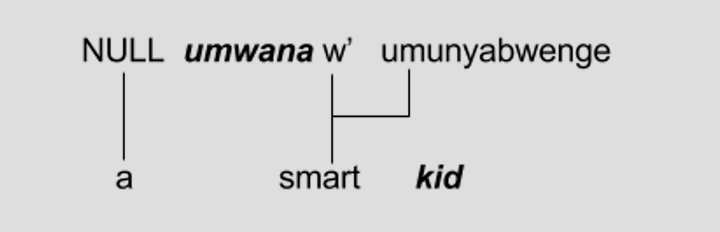
\includegraphics[width=4in]{figures/fig-four.png}
\caption{An alignment in which \textit{``w' umunyabwenge''} is aligned with ``\textit{smart}''}
\end{center}
\end{figure}
\begin{figure}[h]
\begin{center}
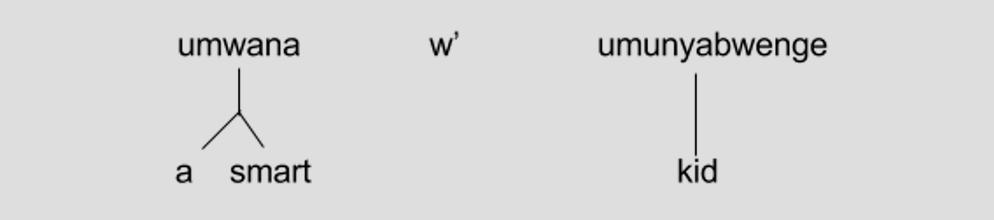
\includegraphics[width=4in]{figures/fig-five.png}
\caption{A graphical representation of another less likely (incorrect) alignment of the sentence pair: ``\textit{a smart kid $|$  umwana w' umunyabwenge}''.}
\end{center}
\end{figure}

To handle this challenge of having several possible alignments for every sentence pair, according to Brown \textit{at al.}\cite[p. 269-270]{brown1993mathematics}, an SMT model has to assign a likelihood probability to each possible alignment. For example, for the \textit{(a smart kid $|$ umwana w' umunyabwenge)} translation pair, both the alignments in Figures $2.4$ and $2.5$ would have bigger probabilities while alignments such as \textit{(a smart kid $|$ umwana(1, 2, 3) w' umunyabwenge)} and \textit{(a smart kid $|$ umwana(1) w'(2) umunyabwenge(3))} would have lower probabilities as they are incorrect, thus less likely to be considered by the translation model.

\section{Phrase-Based Translation Model}
Several SMT systems now use a phrase-based translation model to build phrase translation tables that are more effective than tables generated by word-based alignments \cite[p. 48]{koehn2003statistical}. The reason why phrase-based models outperform word-based models is because phrase-based models break each sentence into phrase segments that are then translated and reconstructed later into the target language. This gives phrase-based translation systems the ability to account for contexts and meanings that words have used alongside some other particular words as opposed to when used alone or with different words. This is taking advantage of statistical probabilities that were in generated from the parallel corpora data used during the training and tuning stages. 

An obvious case in which a phrase-based model would perform better than a word-based model is in the translation of sentences that contain idiomatic expressions. As an example, translating an expression like \textit{cutting corners}\footnote{To cut corners is ``to do something in the easiest, cheapest, or fastest way''\cite{cutcornerscambridge}.} using a word-based translation system would result in the loss of contextual meaning that the words \textit{cutting} and \textit{corners} have when used together in the expression \textit{cutting corners}.

 
\chapter{Developing an SMT Model (Moses)}
Moses is one of the most used SMT systems. It is a complete SMT system with a built-in decoder that can be used with several alignment algorithms. Moses is the SMT system that I used to train my English to Kinyarwanda translation model. In the next section, I describe the steps I followed to develop, train, and test my model using Moses. 
\section{Building a Baseline System}
After successfully installing Moses and other required software (Giza++, Boost, etc), I used it to train my English to Kinyarwanda translation model by using the \textit{King James Version}(KJV) Bible as my English corpus, and the \textit{Bibiliya Yera},  the Kinyarwanda translation of the KJV, as my Kinyarwanda corpus. 

%The following is a snippet of parallel verses extracted from the books of Psalms $119,\:1-2$. The English part is an extract from the \textit{King James Version} Bible and the Kinyarwanda part was extracted from the \textit{Bibiliya Yera}, the translation of the KJV.
%\begin{lstlisting}[breaklines]
    %Blessed are the undefiled in the way | Hahirwa abagenda batunganye
    %Who walk in the law of the Lord | Bakagendera mu mategeko y'Uwiteka
    %Blessed are they that keep his testimonies | Hahirwa abitondera ibyo yahamije
    %And that seek him with the whole heart | Bakamushakisha umutima wose
%\end{lstlisting}

The following is an excerpt of the first three verses of the New Testament in both the Kinyarwanda \textit{Bibiliya Yera} and the English \textit{King James Version} Bible (Matthew 1: 1-3). 
\begin{lstlisting}[breaklines]
1:1 Amasekuruza ya Yesu Kristo, mwene Dawidi, mwene Aburahamu ngaya: | 1:1 The book of the generation of Jesus Christ, the son of David, the son of Abraham.
1:2 Aburahamu yabyaye Isaka, Isaka yabyaye Yakobo, Yakobo yabyaye Yuda na bene se, | 1:2 Abraham begat Isaac; and Isaac begat Jacob; and Jacob begat Judas and his brethren;
1:3 Yuda yabyaye Peresi na Zera kuri Tamari, Peresi yabyaye Hesironi, Hesironi yabyaye Ramu, | 1:3 And Judas begat Phares and Zara of Thamar; and Phares begat Esrom; and Esrom begat Aram;
\end{lstlisting}

As you can see from the above excerpt of a parallel corpus, you need to have two files two equivalent texts in two languages: the target language and the source language. The content in those two files need to correspond line by line. Line 100 in the target language's file should be the translation of line 100 in the file containing the source language. In my case, as I was trying to build an English to Kinyarwanda translation system, I started with two different files, one containing the \textit{Bibiliya Yera} and the other one containing the \textit{King James Version} Bible. When using Moses, the first step in training a translation model is a process called \textit{``Corpus Preparation''}.
%%%%%%%
\subsection{Corpus Preparation}
Corpus Preparation consists of three steps: tokenization, truecasing, and cleaning.

During tokenization, spaces are added between all words and punctuation to make sure that different forms of the same word are counted as one. Without this step, the string ``God'', for example,  would be considered to be different from the string ``God!''. To avoid this kind of behavior that would result in \textit{data sparsity}, the \textit{Moses tokenizer} adds an extra space  in ``God!'' to make it ``God !''; thus, when frequencies of the word ``God'' are calculated, the Moses engine is able to return a correct count that contains all the occurrences of ``God!'', ``God,'', etc.

In the next step, Moses uses a \textit{truecasing} script, also known as the \textit{truecaser}, to calculate the frequencies ratios of how many times a certain word is lower-cased compared to when it is capitalized. This is important as without this step, it would be almost impossible for the translation system to guess if the words at the beginning of a sentence are capitalized because they are normally capitalized (proper names) or if they are capitalized just because they are the at the beginning of their respective sentences.

For example, the word ``God'' and ``god'' have two different meanings and those two meanings should be handled correctly by the translator. However, when ``God'' is used at the beginning of a sentence, the translator can't know for sure if it is capitalized because it is meant to be ``God'' or if it is the word ``god'' that is capitalized because it is at the beginning of a sentence. In this case, the \textit{Moses truecaser} trades off the $100\%$ uncertainty for a statistical guess based on the frequencies of both strings in the corpus. In an instance in which the frequency of the word ``God'' in the corpus is less than that of the string ``god'', all occurrences of ``God'' at the beginning of sentence will changed to ``god'', otherwise there will be no change. This is done for all words in the corpus and it helps to ensure that all meanings associated with capitalization are not all lost during the translation process. 

The last but very important step is the cleaning step. In this step, a sentence pair is removed from the training data if one of its sentences has a character count greater than a set amount, or if the ratio of the character counts of its sentences is not proportional to the calculated or set ratio for the training data. The limiting character count is set according to the structure of the languages that are being dealt with or the quality/size of the parallel corpora being used. 

In my case, I set to the character count to 180, which is very high compared to the ones used in the Moses tutorials that I looked at\cite{koehn2010moses, mosesbaselinesystem}. The reason why I set the limiting character count of my translation system to a larger number is because Bible verses tend to be very long than normal sentences used in conversations and discussions, two major sources of data used in the above-mentioned Moses tutorials.\cite{koehn2010moses, mosesbaselinesystem}.

In addition to that, I am confident that the verse-by-verse translations that I used to train my model are correct as they are from the Bible, and thus have been proofread by humans. In addition, as the main goal of this step is to remove incorrect translations, and I am more than confident in the literary accuracy of training data I used, setting a lower limiting character count for my translation model would not had improved my model at all, it would actually have caused more data scarcity, and that would reduce the overall accuracy of my model.

Below are the first three verses (Matthew 1: 1-3) from the \textit{King James Version} Bible after going through the three steps of the \textit{``Corpus Preparation''} process.
\begin{lstlisting}
1 : 1 The book of the generation of Jesus Christ , the son of David , the son of Abraham .
1 : 2 Abraham begat Isaac ; and Isaac begat Jacob ; and Jacob begat Judas and his brethren ;
1 : 3 And Judas begat Phares and Zara of Thamar ; and Phares begat Esrom ; and Esrom begat Aram ;
\end{lstlisting}

%%%%%%%%%%%%%%
\subsection{Language Model Training}
Target language model training is the following step after corpus preparation. In this step, I used Moses' built-in KenLM 3-gram model tool to construct a target language mode based on my corpus. In this case, as I am working with an English to Kinyarwanda translation, Kinyarwanda is my target language, thus I am going to use the \textit{Bibiliya Yera} corpus file generated the \textit{truecaser}. At this point, there is no need of using the output generated after the cleaning stage of the \textit{Corpus Preparation} process as a language model only depends on the structure of the target language being used, Kinyarwanda in this case, and not to its equivalent translation to the source language,  English in this case. Therefore there is no need to take into consideration the effects of the sentence character count and the limiting ratio used to filter data in the cleaning stage of the \textit{Corpus Preparation} process. After building the Kinyarwanda language model, I used the \textit{Moses binarizing script} to turn the file containing the Kinyarwanda language model into a binary version that loads faster. At this step, I can use it to get the probability that any input sentence is part of the Kinyarwanda according to the language model that I built using data solely from the \textit{Bibiliya Yera}. 
\begin{figure}[h]
\begin{center}
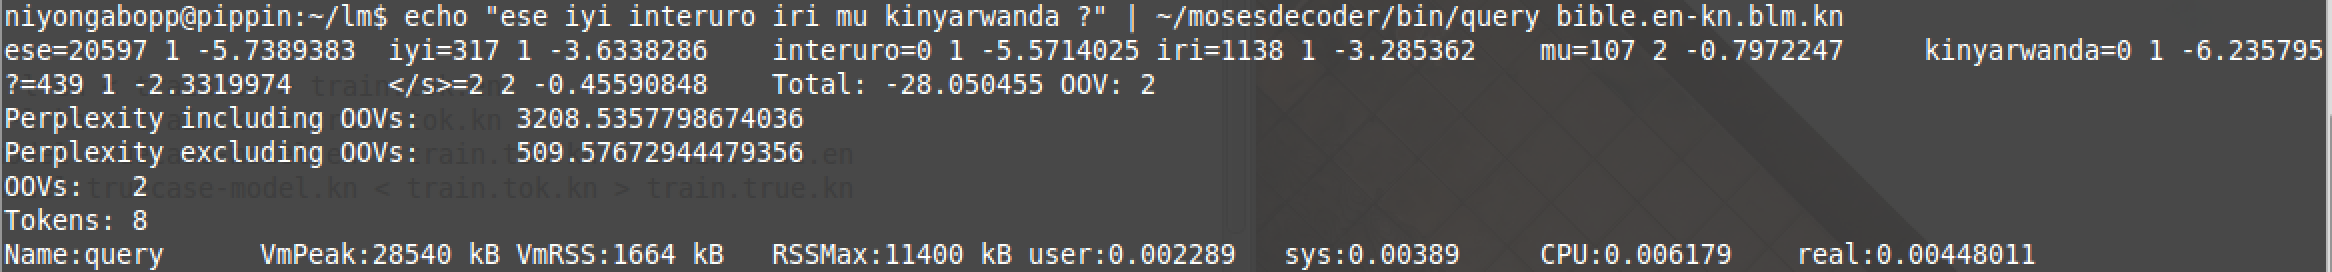
\includegraphics[width=4in]{figures/testing-a-lm}
\caption{Checking if the sentence ``ese iyi nteruro iri mu kinyarwanda ?'' (``is this sentence in kinyarwanda ?'') is indeed in Kinyarwanda according to a language model developed using corpus text from the \textit{Bibiliya Yera}.}
\end{center}
\end{figure}
\subsection{Training the Translation System}
Now that we have trained our target language model, it is time to start training the translation system. For this step, I used Moses default word-alignment tool called Giza++. After running the commands for this step, \textit{Moses} generated a \texttt{Moses.ini} configuration file that can be used to translate any English sentence to Kinyarwanda. However, at this point, there are two main issues that must be looked at. The first one is that translation takes a long time; to fix this we need to binarise the \textit{phrase and reordering tables}. The second one is that weights in our model configuration file are not adjusted, i.e.: they are dependent to the Bible data we used in training the model. In the next subsection, I talk about the process of tuning our model to make it more balanced and less dependent on the data used to train it.
%%%%%%%%%%%
\subsection{Tuning the Translation Model}
To tune our model, we need a separate small parallel corpus of high quality to add statistical variety to our model. The tuning process is important as it helps in making the translation model more balanced and less biased towards the data that was used during the training step. For example, as we only used data from the Bible, our model has only seen sentence structures, expressions, and words' combinations that are common in the Bible and nothing else from the commonly used conversational and/or formal language. Therefore, to make our model more efficient, it is crucial that we tune it using data that is very different from the Bible. As I couldn't easily find good-quality English data that is also translated in Kinyarwanda, I used the Rwandan constitution as it is freely-available on the web both in Kinyarwanda and in English. In the tuning process, as in the training process, I completed the steps of the \textit{corpus preparation} process on the tuning corpus data before using it. I ran the tuning process by using the minimum error rate training (MERT) algorithm\cite{och2003minimum}, the default option in \textit{Moses}\cite{mosesfactoredtraining}. I also performed this step in a newly created folder to avoid overwriting my previous model's configuration files.


\subsection{Binarising Phrase and Reordering Tables}
Once the tuning process is over, it is advised to binarise the \textit{phrase and reordering tables} in your translation model by using the Moses' built-in tools specialized for this process\cite{mosesbaselinesystem}.
\begin{figure}[h]
\begin{center}
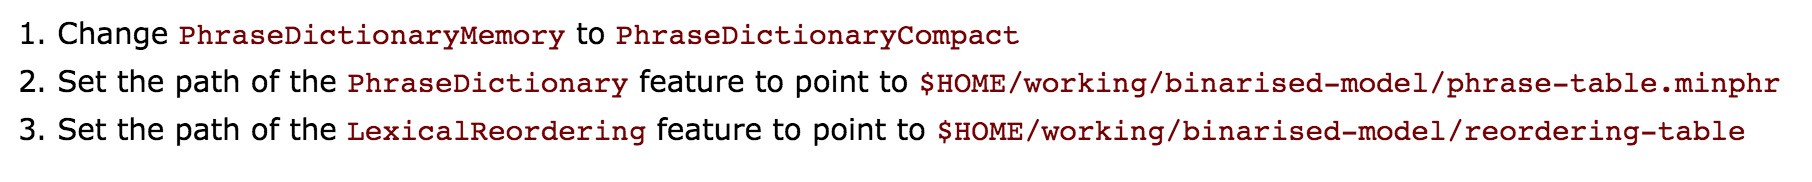
\includegraphics[width=4in]{figures/change-variables}
\caption{Examples of changes made to the \texttt{Moses.ini} configuration file to make sure it correctly points to the \textit{binarised} tables and the \textit{binarised} model directory.}
\end{center}
\end{figure}
\subsection{Testing the Translation Model}
Now that we have completed the basic steps of building, training, and tuning a translation model using \textit{Moses}, we can use it to do some simple translations. To do this, all you have to do is running terminal command, and that way you can translate a file containing sentences in English to Kinyarwanda. The sentences in the input file have to be in the same format as the ones in parallel corpora used in the training and tuning stages.

Below is the content of the English input file that I used to test my translation system followed by the Kinyarwanda file content that was generated the translator. \newline


\lstinputlisting[numbers=left]{files/input.txt}
\lstinputlisting[numbers=left]{files/output.txt}
\clearpage
\section{Translation Results}
As it can be seen from the results on the previous page, my translation system is still struggling with the translation of content that is not from the Bible. It can also be seen that it is almost incapable of translating long sentences as the one in line $5$. However, I am still hopeful that it can be improved by using more data. The data I used to train and tune  my translation model is like a drop in the ocean compared to the recommended quality and size as stressed by Och\cite{och2005statistical}.

It should also be noticed that even though the quality of my translation results if of low quality, the results I am getting are consistent with the parallel corpora I used to train and tune my translation model. As I used the Bible in the training process, one should expect my model to do well on translating sentences from the Bible. To a certain degree, that is what my model is doing but with an slightly lower accuracy rate. I suspect that is mainly caused by two reasons. 

The first one is that SMT systems work by using mathematical probabilities and decoding algorithms and not by directly looking up of each sentence in a large catalog of translations. The benefits of this is that SMTs systems are capable of translating sentences they have never seen before. However this comes at a cost that in some instances, the SMT model will return an incorrect translation for a sentence contained in the data that was used to train it.

\lstinputlisting[numbers=left, caption={Translation output of the English text on page $18$ when using a translation model both trained and tuned using content from the Bible.}]{files/example6.txt}
%\footnote{I used Psalms 119 because it is the longest chapter in the Bible and because it is made up of shorter sentences.}


The second reason why my translation isn't doing well as expected at translating sentences from the Bible is because I used data from the Rwandan Constitution in the tuning process. I did that hoping that tuning my translation model using external data would help improve the overall performance of the model, however it is hard to judge that with the results I have right now because my corpora sizes are too small to have a significant impact. The only thing that I am sure of is that tuning reduced the accuracy of my model for translations of sentences from the Bible. This is illustrated by the sentences in the example in Listing $3.1$ which are better translations of the input file than the results displayed on page $18$.


Another important thing to notice is that my translator, like other SMT-based translation systems, is incapable of inferring the difference of homonym words. For example, when I tried to translate ``It’s not that I’m so smart, it’s just that I stay with problems longer'', a quote attributed to Albert Einstein, my translator translated the word ``just'' as ``umukiranutsi'', the Kinyarwanda translation for ``a fair'' or  `` an impartial'' person! This shows that even though SMT-based translation systems perform better than rule-based systems, SMT is still inferior to human translation especially when it comes to these kind of situations in which words with the same spelling have more than one meaning.
\clearpage

\chapter{Improving SMT Model}
\section{Gathering More Data} % PROVIDE 5 CITATIONS TOTAL
The first thing I did to improve the SMT model described in this paper is to gather more high-quality Kinyarwanda | English translation data ad formatting it in the right way so that I could add to data from the Bible that I already had. To do this, I started by gathering translated texts from various on-line sources such as news articles, blog posts, encyclopedia entries, etc. But this wasn't enough as most of these translations either contained some mistakes that I had to manually correct or they were not ready for direct use as they were incorrectly formatted and I had to copy paste them into files, and check line by line to make sure they are well-formatted; and this was quite a lot of work for one person, and there was no going around it because from what I understand, having incorrect data would corrupt the translation model and this would easily lead to several erroneous and inaccurate translation results. 
\section{Kinyarwanda Online}
Having realized that I couldn't possibly complete the process of gathering data on my own, I went ahead and set up a translations crowd-sourcing website. On the website provided, I provided a list of the most used English sentences, I asked Kinyarwanda and English bilingual users to provide translations to as many sentences as they can. This initiative did not go well as I planned as only few people participated. The website is still on-line at this link:  \url{http://kinyarwanda.online/}, and I am still waiting for more translations to added by users with the hope that one day I or someone else can use the data gathered from the website to develop a new Kinyarwanda | English translation system and/or help improve existing ones such as \textit{Google Translate}\footnote{Kinyarwanda is one of the languages under development by Google Translate. Volunteers can contribute by providing or validating translations at \url{https://translate.google.com/about/intl/en_ALL/contribute.html}} and \textit{SmartRwanda}\footnote{\url{https://smartrwanda.org/translate}}.

\begin{figure}[h]
\begin{center}
\captionsetup{justification=centering}
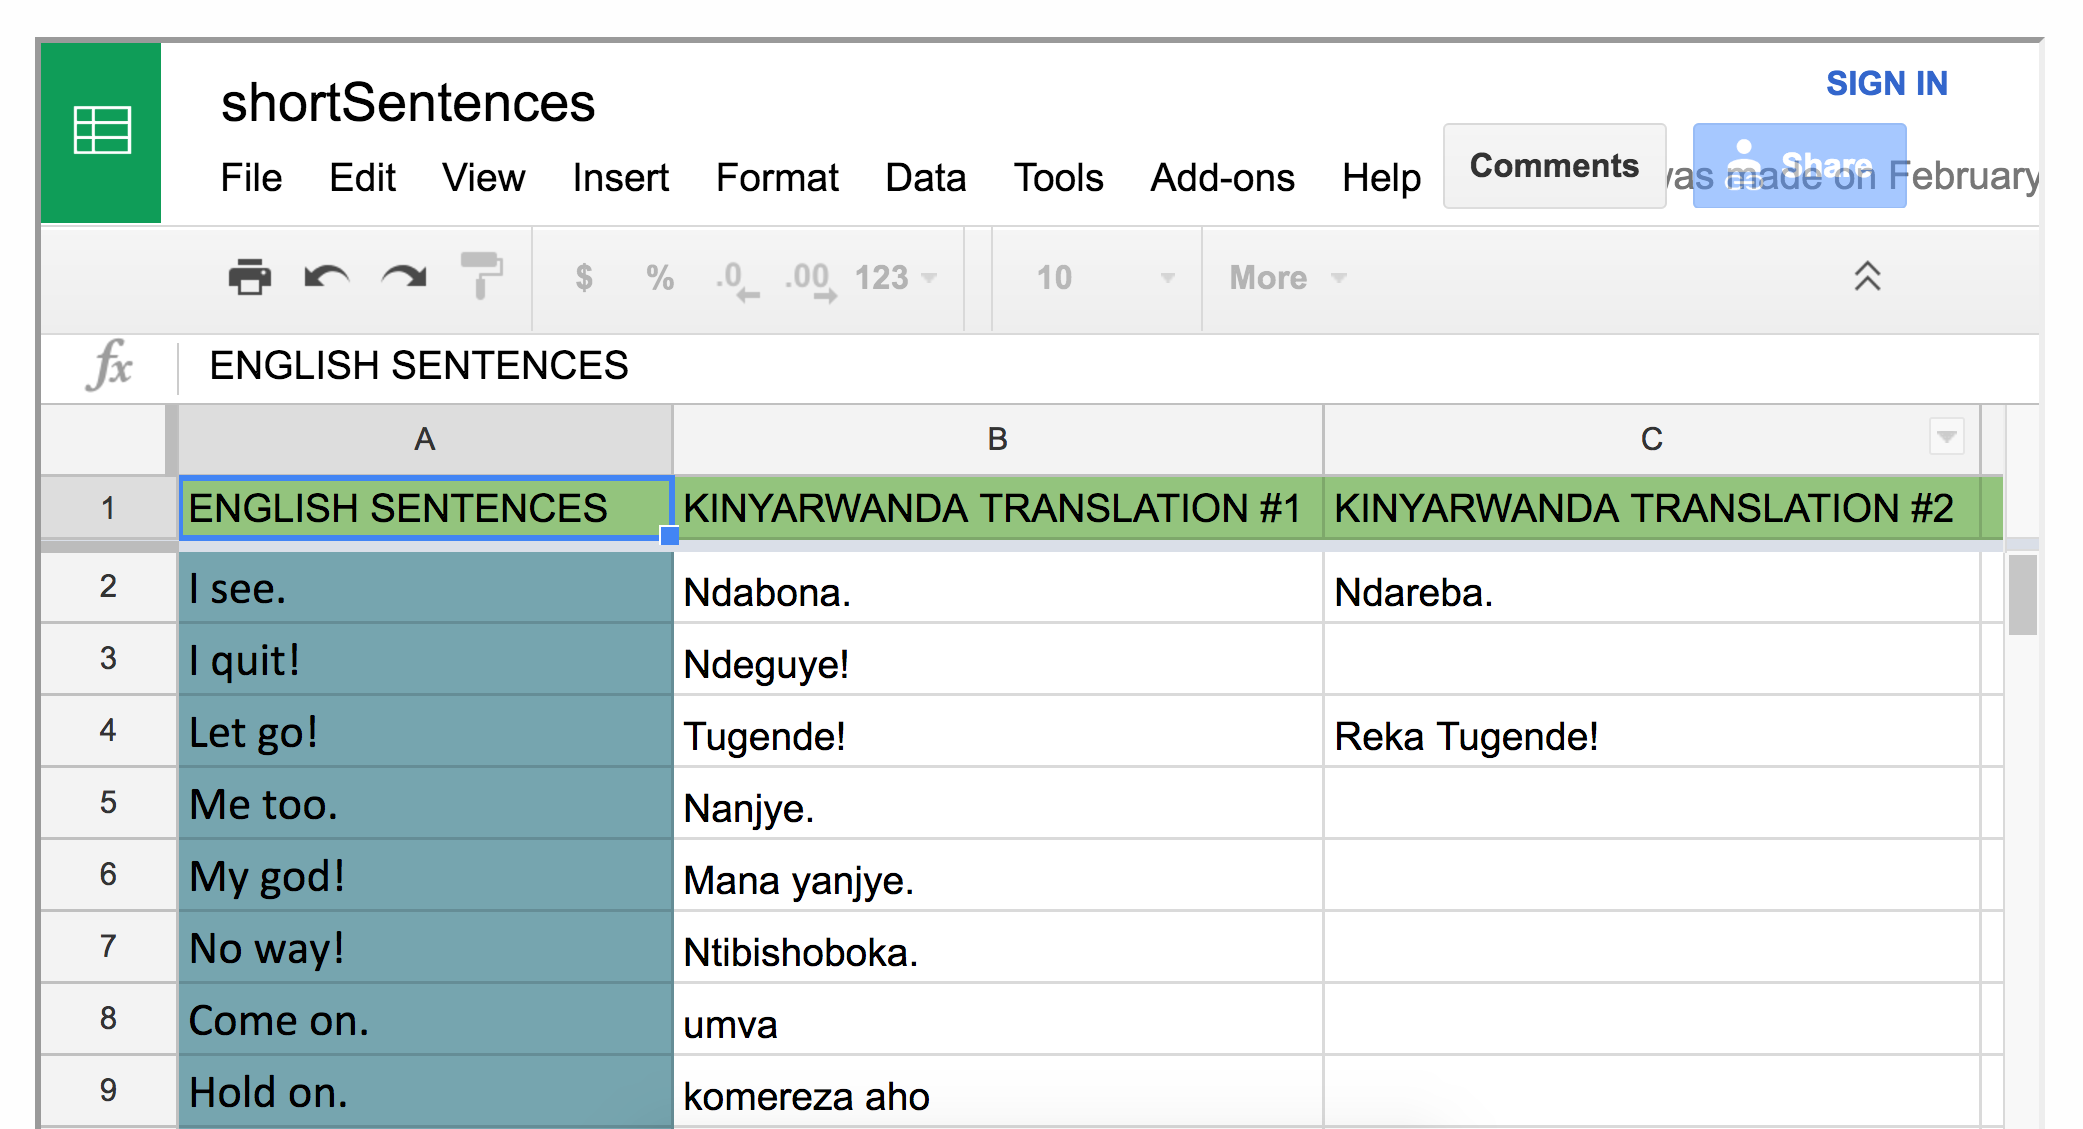
\includegraphics[width=6in]{figures/kinyarwanda-online-spreadsheet.png}
\caption{A preview of the spreadsheet containing crowd-sourced translation data. 
Image Source: \protect\url{http://kinyarwanda.online/translate/}. Screenshot taken on March 29, 2017.}
\end{center}
\end{figure}
\chapter{Rule-Based Machine Translation} % PROVIDE 5 CITATIONS TOTAL
After realizing that finding Kinyarwanda | English translation data couldn't possibly be achieved with the time and other resources I had allocated for this project, I started working on a rule-based machine translation(RBMT) model. To develop an English to Kinyarwanda RBMT model, I used a word-by-word translation dictionaries from the \textit{SmartRwanda} translation engine\footnote{https://smartrwanda.org/translate}; then I wrote a python program that takes an English sentence as input, lowercase it, split it into a list of words, and for each word in that list, check to see if it is in the translation dictionary, if yes translate it, and if not, just return it as it is. After this process is over, the resulting translated and non-translated words are all joined together into a pseudo-Kinyarwanda sentence and returned as a string.

Even though the concept of RBMT sounds easy that it can be summarized and explained in a few sentences; for the sake of clarity, I will split and describe it in two sections: data collection and model implementation. 
\section{Collecting Translation Data}
First, I dealt with the challenge of getting a decent amount of translation data of words and expressions. Even the data that I got from \textit{SmartRwanda} contained false translations and translations and several errors. To save time, I ignored the errors and used it anyway because I was more interested in analyzing the behavior of the RBMT model more than I was interested in the complete accuracy of the translations results.
\section{Implementing the Translation Program}
Second, I implemented a Python program\footnote{The source and data files I used to make the translator are publicly available and accessible on my Github account. Link: \url{https://github.com/npatrick96/kinyarwandaRBMT}.} for the actual translation process. My implementation of the program consisted of three main components. The first step cleans the input by lower-casing it, and then removing all trailing spaces and punctuations. In the second step, the cleaned input is translated to Kinyarwanda word by word by looking up each word in the translation dictionary. In the third step, the program attempts to improve the translation by following the provided translation rules by adding, modifying, re-arranging or removing some parts of the output Kinyarwanda sentence to be returned by the program.

From my experience, the first and second components are easy to implement and not as important as the third one when working with a non-trivial implementation of an RBMT model. In my case, working on the third component was additionally challenging due to both my limited experience in the study of linguistics (incl. both English and Kinyarwanda), and the scarcity (and poor quality) of the translation data I was working with. However, despite these constraints, I managed to program simple rules to handle a few useful cases such plural forms in English and noun + adjective alignments plus ignoring articles in Kinyarwanda. This helped in improving the translation results as it can be seen in the example shown below.
\begin{lstlisting}
English sentences to translate to Kinyarwanda.
1. Hello, my name is Patrick. Good morning!
2. laws are heavier than stones

Translations before the implementation of the third component.
1. hello , my izina is patrick . cyiza igitondo ! 
2. laws kuri heavier kuruta stones

Translations after the implementation of the third component.
1. hello , my izina is patrick . igitondo cyiza !  
2. itegeko kuri heavier kuruta ibuye 
\end{lstlisting}
From the previous example, one notices that even though the implementation of additional rules can improve the overall quality of translation results, one ought to be careful when implementing these rules as they can easily break the existing structure of the whole model. Therefore each additional rule should be examined and tested to make sure it does not conflict with existing rules.  If it does, it is necessary to make sure that it actually improves the existing model. For example, after I added a new rule that appends an ``s" to the end of each English word and used it to create a new vocabulary entry to handle plural forms, I realized that this rule doesn't help at all with words with irregular plural forms, and that it was causing translation errors for English words whose singular Kinyarwanda translations are very different from their plural translation. 

For example, the translation of ``law" is ``itegeko", but as I only have an entry for the word ``law" and not its plural form ``laws", my RBMT model wasn't able to translate ``laws" before I added a rule that took care of plural forms. However, even though the final translation of ``rules" as ``itegeko" is slightly incorrect\footnote{The grammatically-correct Kinyarwanda translation of ``laws" is ``amategeko".}, it is definitely better than having no translation at all.  

Another example on the usefulness of extra rules can be seen in the translation of ``good morning". In Kinyarwanda, unlike in English, adjectives come after the nouns they are describing. Therefore, with ``good" = ``cyiza" and ``igitondo" = ``morning", the correct translation of ``good morning" is ``igitondo cyiza" instead of ``cyiza igitondo".

To program this into my model, I created a list that contained adjectives, and when re-joining translated words into a new sentence, the program had to check if the current word being added to the sentence was an adjective and switch it with the following one. However this posed a few challenges as in the case in which two or more adjectives are used to describe the same word or the case in which the adjective is used at the end of a sentence, e.g.: the car is fast. These cases or similar ones can be handled by writing new rules or existing ones or ignored if they don't occur as often or if their impact on the translation quality is insignificant.
%%%%%%%%%%%%%%
\chapter{MT Battle: SMT Versus RBMT} % PROVIDE 5 CITATIONS, 8 TOTAL
To compare the two \textit{Machine Translation}(MT) models discussed in this paper: SMT (Statistical Machine Translation) and RBMT (Rule-Based Translation), it is important to understand how both models are implemented, what kind of raw data they require, and what kind of results to expect when using these two MT models. In addition to that, it is crucial to take into consideration the amount of effort it would take to improve or scale each of the two models. 
\section{Data Usage and Model Implementation}
The first main difference between SMT and RBMT is the type of data used in their implementations. The Moses SMT model that I implemented uses parallel corpora (translated sentences pairs) from both languages as primary input data. On the other hand, the RBMT model that I recently implemented using \textit{Python} uses a Kinyarwanda | English dictionary containing mostly single words and a few 'short expressions'. 

These differences in the kind of data used dictate how each particular model work and how it is implemented. As I explained in chapter one, SMT models translate a sentence by using statistical patterns derived from analyzing the parallel corpora data used as input\cite{Forcada2011}. Therefore it is possible that a good SMT model would correctly translate a sentence even if it has not seen it before\cite{Forcada2011}. Au contraire, RBMT models work by translating each word in the provided sentence thus making it impossible for an RBMT-based model to fully translate a sentence that contains a word that is not in its translation dictionary. This and other advantages and/or limitations of RBMT models versus SMT models are discussed in the following section that focuses mainly on the efficiency and the effectiveness of each model.

\section{Efficiency and Effectiveness}
According to the \textit{Cambridge English Dictionary}, the word \textit{efficiency} is defined as ``the condition or fact of producing the results you want without waste"\cite{cambridgeefficiency}, and \textit{effectiveness} is defined as ``the ability to be successful and produce the intended results"\cite{cambridgeeffectiveness}. Comparing SMT and RBMT based on \textit{efficiency} and \textit{effectiveness}, one may be tempted to conclude that SMT is the absolute winner. But by looking closely, one starts to realize that even though SMT is more efficient than RBMT as there is no wasted effort that goes into training an SMT model versus an RBMT model\footnote{In the training and tuning process of an MST model, the aim of each step is to improve the translation model. RBMT models on the other hand, contain several repetitive, and sometimes conflicting, conditional rules that may results in reduced efficiency in many cases.}, it is not easy to judge the effectiveness of both models because of the definition of this word itself. 

To get the full picture, it is crucial to define the ``intended results" before one starts comparing the effectiveness of these two models.  In this case, “intended results” can either be set based on the intended usage of each model, or adjusted to be slightly the same (therefore comparable) for both models. As the latter case is simpler, and therefore most likely easier to analyze, let's assume that both models have analogous ``intended results". That is, we are choosing to assume that we have similar (comparable) standards that we will use to evaluate the results of both models. If the intended goal of the translation model was to return a sentence that makes sense in the target language, SMT would be the absolute winner as it take into consideration the context in which words or groups of words are used. However, if all we cared about was the number of translated words in output sentence, RBMT would likely win this round because what an RBMT model does is to look up a word or an expression from a translations dictionary and return its equivalent translation of it exists. 

For example, if the dictionary contained all possible words, an RBMT model would translate all words, but that doesn't mean that the returned translation is correct as that solely depends on how the implementation of translation rules, and other factors such as words alignment, language grammar, etc. As you can see from the two possible scenarios discussed above, the effectiveness of SMT versus RBMT models depends on not only depends on the kind (and size) of input data used and the model implementation, but also the ``intended results".

\section{Improvement and Scalability}
Now that that I have talked about overall performance and model results, it is imperative that I discuss how both models can be improved and developed to be used on a larger scale. There are two obvious ways in which these two models can be improved. The first one is by improving the quality and increasing the quantity of the data used as input, and the second one is by enhancing the internal implementation of each model. From my experience, the easier and more effective way to improve an SMT model is by using more good-quality data in the training, tuning, and testing stages. 

Au contraire, improving an RBMT model requires revising and adjusting the existing code that handles the translation process and adding new use-cases if necessary. This can be challenging for anyone like me who is not a linguistics expert. During this project, even though I was dealing with Kinyarwanda and English, two languages that I speak and write comfortably, I was surprised by the amount of grammatical and lexical rules I didn't know or understand well enough when I tried writing code to improve my English to Kinyarwanda RBMT model.


% cite 3 sources in below paragraph
In addition to that, one can imagine the inconvenient complications that can be caused the by having to implement manually all the rules in an RBMT model. To that, add the cumulative burden of dealing with multiple languages unlike in SMT models where translations can be re-used for different languages, translation rules in RBMT can differ when from one language to another\cite{Forcada2011}. For example, the rules used to translate English to Kinyarwanda would be very different from the rules of translating English to Chinese. Imagine writing thousands lines of code for each languages-pair, and starting over again for another pair. 

A system like this is not only repetitive and inefficient, but also difficult to scale. For example, if you had an existing working RBMD based translation system that supported multiple languages, and you all want is to add a new rule to one of the languages, you would have to check all the other rules in all the pairs containing that language and make sure that none of those rules would conflict with the new rule; and if such rules exist, you would either have to modify them or delete them. This is why translation services such as \textit{Google Translate} use SMT instead of RBMT\cite{koehn2003statistical}, and many \textit{Machine Translation} scholars are spending more time doing research related to Statistical Machine Learning and its application in natural language translation\cite{koehn2007moses}. 

 
\chapter{Concluding Remarks}


First of all, before talking about what I thought about the overall progress of this project and what I think of the English to Kinyarwanda translation model that I current have, I think it is important that I first talk about some important decisions that I have had to make when working on this project.

\begin{itemize}

    \item \textbf{Why English to Kinyarwanda?} Why not Kinyarwanda to English? The reason why I chose to work on an English to Kinyarwanda translation model and not the other way around is because of need. Most Rwandans who would want to use a Translator would most likely use to translate content (books, articles, manuals instructions, etc.) from English to Kinyarwanda or from other popular languages to Kinyarwanda. I chose to work with English because it is one of the three official languages in Rwanda, the others being French and Kinyarwanda. English is also the language used in education, from primary schools to universities\cite{Samuelson2010}. As for the reason I chose to work on an English to Kinyarwanda translator, and not the other way around, that can be explained by the fact that Rwanda had been an oral society for most of its existence, and there aren't so many writings in Kinyarwanda that one would possibly want to translate to another language\cite[p. 59]{adekunle2007culture}. Even the majority of the ones that exist aren't digitalized or freely-available online, which makes using them or simply accessing even more challenging. %Therefore, out of pragmatic reasons, I chose to work on the English to Kinyarwanda model because, if it was to be developed into a stable/decent application, it is likely to be used than its Kinyarwanda to English counterpart.
    \clearpage

    \item \textbf{Why the Bible and the Constitution?} I chose to use the Bible as my training data because it is the only large body of text that has both English and Kinyarwanda translations that I could find online. I used the Rwandan constitution for tuning as it is an official document that has good-quality content for both Kinyarwanda and English. I also used it because, as a non-religious text, it offers a good variation to the content from the Bible that I had used in the training process. 

    \item \textbf{What is the main challenge that I faced?} The main challenge that I faced is data sparsity. Kinyarwanda is not a popular language by any metric. Even though it is estimated that Kinyarwanda is spoken by around 20 million people, the majority of them live in Rwanda and its neighboring countries (Burundi, Uganda, Tanzania, and Democratic Republic of the Congo), and it isn't used elsewhere in the World\cite{kayigema2010loanword}. That and the fact that Rwanda used to be an oral society and still is to some degree, guarantees that getting Kinyarwanda data or  Kinyarwanda software is almost impossible. According to Samuelson \etal, despite its massive use in Rwanda and neighboring regions, ``mass literacy in Kinyarwanda remains weak''\cite{Samuelson2010}. One of the consequences that I faced when working on my project is that Moses, the SMT system that I used didn't even have a Kinyarwanda \textit{tokenizer}. I had no choice but to use the default (English) one and hope for the best! 

    \item \textbf{Why start with statistical machine translation?} I initially chose to use SMT as opposed to RBMT because that SMT systems are easy to work with and are easily scalable compared to rule-based translation models\cite{och2005statistical}. As my end goal for this project is to turn it into an open-source system that other people can contribute to, scalability was very important when taking this decision. I thought that implementing the translator using an SMT system would make it possible and easier for people, with different levels of technical expertise and Kinyarwanda proficiency, to contribute to the project either by providing more training data (in forms of translated texts), correcting translations generated by the translator, or writing code for translation tools specialized for Kinyarwanda. 

    \item \textbf{Why Moses?} As I did not have any previous experience working with SMT systems, this wasn't an easy choice. I had to try all the popular SMT systems and decoders and decide which one to use. I tried Joshua, Cdec, and Moses. Unfortunately, Joshua and Cdec ran into compiling issues on my computer, and despite my multiple attempts, I couldn't get them to work past the tutorial stages found on their websites. With that, I had only one choice left: Moses. However, even though I had no other choice when I started using it, through the process of using Moses to develop my English to Kinyarwanda translation model, I have come to appreciate the fact that it has a lots of documentation and supporting documents that are easily-accessible and freely-available online.
    
    \item \textbf{What is next?} As I have unsuccessfully tried to gather enough Kinyarwanda | English translation data on my own, my plan is to make this project open-source by making all the source and data files publicly available on the project website\footnote{\protect\url{http://kinyarwanda.online/}}. That way anyone working on a similar project can access it and contribute to it at the same time. I will also continue to work on this project in my free time and I intend to use all means in my disposition (social media, project website, presentations, etc) to ask more people to contribute to small-scale Kinyarwanda translation projects like this one and to large-scale translation initiatives such as \textit{Google Translate}.
    
    %For now, my next goal is to try to get as much Kinyarwanda data as possible. As I already mentioned, it is not that difficult to get English data. The real challenge is getting Kinyarwanda data in right format (\texttt{.txt} file, line by line sentences, character count not too small or too large, etc.). However, what is even more difficult is getting Kinyarwanda data that has correct, human-proofread, line by line, equivalent English translation. Regarding this, my plan going forward is to set up a website that will crowd-source translations by generating English text line by line and asking users to translate it. Hopefully, I will get a decent amount of data this way. In addition to this, I intend to keep looking for and collecting English $|$ Kinyarwanda data and adding it to my training corpus, that way I hope to keep improving my model. 
\end{itemize}


To sum up, having asked and answered these important questions, all I have to add is that despite all the challenges I have faced when working on this project, I have more determination now more then ever. I am more determined because I have learned a lot by working on this project, and the experience in itself has been more rewarding than I ever could have hoped for when I embarked on this journey.

%and because I know that as long I keep working on this project, the quality of my translation model results will keep improving.  % then conclude




%\usepackage{fancyvrb}
%now enable appendix numbering format and include any appendices
\appendix
\chapter{Code Reference: \texttt{Moses.ini}}
\texttt{Moses.ini} file generated by my English to Kinyarwanda translation model after training and tuning\footnote{Using the minimum error rate training (MERT) tuning algorithm.} it using data from the Bible \footnote{The \textit{King James Version} Bible for English and the \textit{Bibiliya Yera} for Kinyarwanda.} and the Rwandan Constitution respectively. \newline
\lstinputlisting[numbers=left]{files/moses.ini}


%\section{Examples of configuration files generated by Moses}
%\underline{\textbf{Examples of configuration files generated by Moses.}}

%\lstinputlisting[numbers=left, caption={The \texttt{Moses.ini} file generated after training my English to Kinyarwanda translation model using data from the Bible (\textit{King James Version} for English and \textit{Bibiliya Yera} for Kinyarwanda).}]{files/moses1.ini}


%\texttt{Moses.ini} configuration file generated after tuning the translation model using Psalms 119, the longest chapter in the Bible both by words and verses count according to \textit{Pathos.com}. \newline
%\lstinputlisting[numbers=left]{files/moses2.ini}

%\lstinputlisting[numbers=left, caption=This is the final \texttt{Moses.ini} file generated after tuning my English to Kinyarwanda translation model using data from the Rwandan Constitution.]{files/moses1.ini}
 

\chapter{Code Reference: \texttt{translator.py}}
A simple \textit{Python} program that I implemented for my RBMT model. An updated copy of this file and other data files are hosted and publicly available in a \textit{Github} repository accessible at this link: \url{https://github.com/npatrick96/kinyarwandaSimpleTranslator}. \newline
\lstinputlisting[numbers=left]{files/translator.py} %\texttt{translator.py}

%next line adds the Bibliography to the contents page
\addcontentsline{toc}{chapter}{Bibliography}
%uncomment next line to change bibliography name to references
%\renewcommand{\bibname}{References}
\bibliography{refs}        %use a bibtex bibliography file refs.bib
\bibliographystyle{plain}  %use the plain bibliography style

\end{document}

